\documentclass[12pt, notitlepage]{article}   	% use "amsart" instead of "article" for AMSLaTeX format
\usepackage{geometry}                		% See geometry.pdf to learn the layout options. There are lots.
\geometry{a4paper}                   		% ... or a4paper or a5paper or ... 
%\geometry{landscape}                		% Activate for rotated page geometry
\usepackage[parfill]{parskip}    		% Activate to begin paragraphs with an empty line rather than an indent
\usepackage{graphicx}				% Use pdf, png, jpg, or eps§ with pdflatex; use eps in DVI mode
								% TeX will automatically convert eps --> pdf in pdflatex

\usepackage{hyperref}

%Use for images
\usepackage{graphicx}
\graphicspath{ {./images/} }

%SetFonts

\usepackage[T1]{fontenc}
\usepackage[utf8]{inputenc}

\usepackage{tgbonum}

%SetFonts

\title{
	\textbf{
		Mini-Quiz 4
	} \\
	\large BIOL 4301/6301 \\
	\large September 26, 2019 \\
}

\date{\vspace{-5ex}}

\def\wl{\par \vspace{\baselineskip}}

\begin{document}

{\fontfamily{phv}\selectfont %select helvetica (code = phv)

\large{Name:}

{\let\newpage\relax\maketitle}

\section{\small{A recent article by Bastin et al. (full citation below) posited that
the Earth could hold an additional 0.9 billion hectares of trees. The authors
then used carbon cycle equations for NPP to suggest that this could result in an increase
in carbon stored on land by 205 Gt (see Figure 1 below). 
The authors argue could drastically offset human emissions (300 Gt to date). However, this
paper has been criticized for not considering other carbon cycle and non-carbon cycle
impacts to ecosystems. Use the back of this page to create a systems diagram 
to explore what these impacts might be. From your diagram,
do you support reforesting the Earth; why or why not?}}

\small{Figure 1. Potential increase in global tree cover}

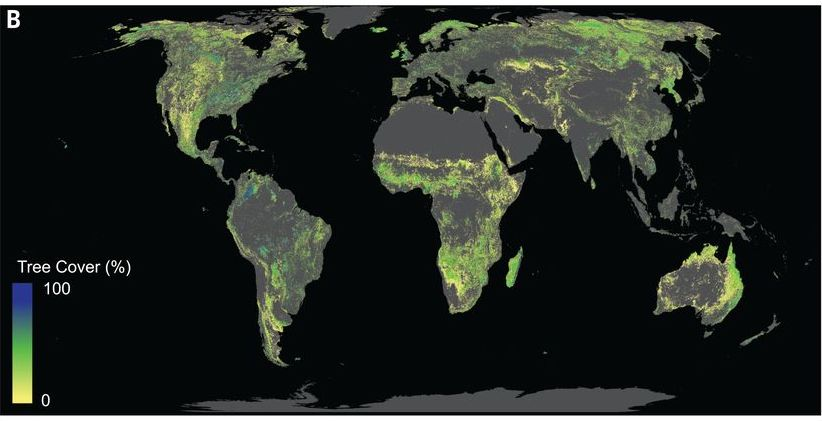
\includegraphics[scale=0.35]{Bastin_fig2.jpg}

\small{This map shows the potential increase in global tree cover that could be observed with a
mass reforestation of the Earth.}

\small{Bastin J-F, et al. 2019. The global tree restoration potential. Science 365: 76 – 79.}


} %end font selection

\end{document}